\documentclass[t]{beamer}
\usepackage[portuguese]{babel}
\usepackage[utf8]{inputenc}
\usetheme{Berkeley}
\usecolortheme{seahorse}

\addto\captionsportuguese{
	\renewcommand{\figurename}{Fig.}
	\renewcommand{\tablename}{Tab.}
}

\title{Meios de Comunicação}
\subtitle{Como podemos trocar dados entre dispositivos.}

\AtBeginSection[]
{
	\begin{frame}
	\frametitle{Sumário}
	\tableofcontents[currentsection]
\end{frame}
}

\begin{document}

\frame{\titlepage}

\begin{frame}
\frametitle{Sumário}
\tableofcontents
\end{frame}

\section{Comunicação}

\begin{frame}{Como nos comunicamos}
\begin{itemize}
	\item Remetente
	\item Mensagem
	\item Emissor
	\item Código
	\item Meio
	\item Ruído
	\item Receptor
	\item Destinatário
	\item ..
\end{itemize}
\end{frame}


\begin{frame}{Como nos comunicamos}
Modelo de comunicação de Shannon e Weaver
\begin{figure}
	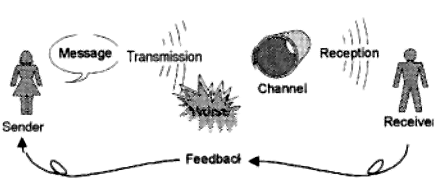
\includegraphics[width=\linewidth]{Shannon-Weaver_model}
	
	\scriptsize Fonte: Claude Shannon e Warren Weaver, "The Mathematical Theory of Communication", University of Illinois Press, Urbana, IL, 1949
\end{figure}
\end{frame}

\section{Tecnologias}

\begin{frame}{Tecnologias para comunicação}
Modo de comunicação
\begin{itemize}
	\item Curta distância
	\item Longa distância
	\item Híbridas?!
\end{itemize}
Tipo de comunicação
\begin{itemize}
	\item Com fio
	\item Sem fio
\end{itemize}
Tipo de rede
\begin{itemize}
	\item LAN
	\item WAN
\end{itemize}
\end{frame}


\begin{frame}{Opções de comunicação}
Algumas opções disponíveis
\begin{itemize}
	\item Cabos: Jumpers, Ethernet e outros.
	\item Infra-vermelho
	\item NFC (Near Field Communication)
	\item Bluetooth v2, v3, v4, v5, A2DP e BLE
	\item Rádio-Frequência
	\item ZigBee
	\item WiFi a, b, g, n, ac e WiFi Direct
	\item 2G, 3G, 4G, 5G
	\item LoRa, Sigfox, NB-IoT, EC-GSM-IoT, LTE Cat-M1, RPMA e vários outros
\end{itemize}

\end{frame}

\begin{frame}{Opções de comunicação}
Infra-vermelho
\begin{itemize}
	\item 1m ou mais
	\item 15 a 30 graus para transmissão
	\item 15 graus para recepção
	\item 2.400 a 115.200 bps no início
	\item Atualmente suporta até 10 Gbps para serviços de broadcasting
\end{itemize}

\end{frame}

\begin{frame}{Opções de comunicação}
NFC
\begin{itemize}
	\item 4 a 10~cm
	\item 0.4Mbps
\end{itemize}
\end{frame}

\begin{frame}{Opções de comunicação}
Bluetooth
\begin{itemize}
	\item 2.4 GHz ou 5GHz
	\item Saída 36.3 a 585.6 kbps com link de 1Mbps no padrão inicial
	\item Recomendação de 10~m, com máximo de 100~m e distância para comunicação.
	\item Hoje suporta 2Mbps ou mais caso use 5GHz
	\item Também permite alcance e mais de 400~m em alguns casos com alto consumo de energia.
	\item Bluetooth Low Energy~(BLE) é otimizado para IoT
\end{itemize}
\end{frame}


\begin{frame}{Opções de comunicação}
ZigBee
\begin{itemize}
	\item 20 a 250~kbps
	\item 1 a 100~m
	\item Arquitetura de rede tipo Mesh
\end{itemize}
\end{frame}

\begin{frame}{Opções de comunicação}
WiFi
\begin{figure}
	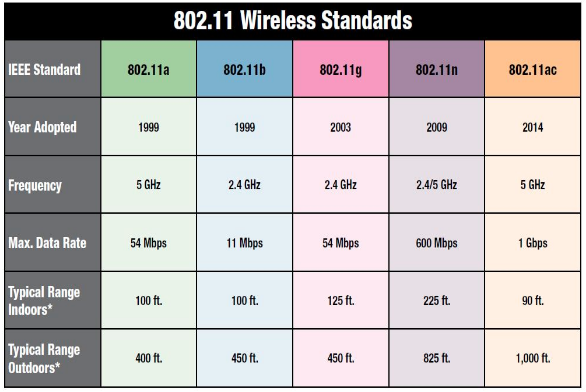
\includegraphics[width=\linewidth]{wirelessstandards}
\end{figure}
\end{frame}

\begin{frame}{Opções de comunicação}
Comparativo
\begin{figure}
	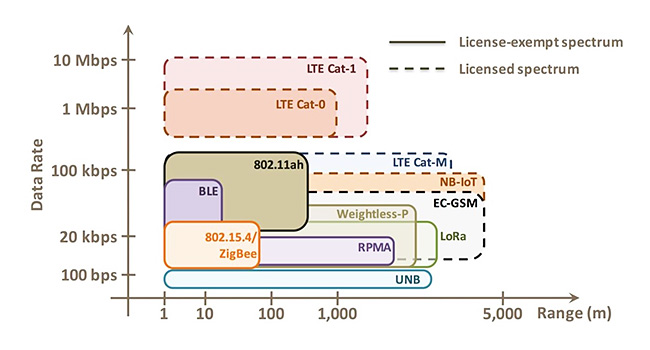
\includegraphics[width=\linewidth]{chart-range-vs-data}
\end{figure}
\end{frame}

\section{Roteamentos}

\begin{frame}{Roteamentos}
Tipos de roteamentos
\begin{itemize}
	\item Unicast
	\item Multicast
	\item Broadcast
	\item Anycast
	\item Geocast
\end{itemize}
\end{frame}

\begin{frame}{Roteamentos}
Unicast
\begin{figure}
	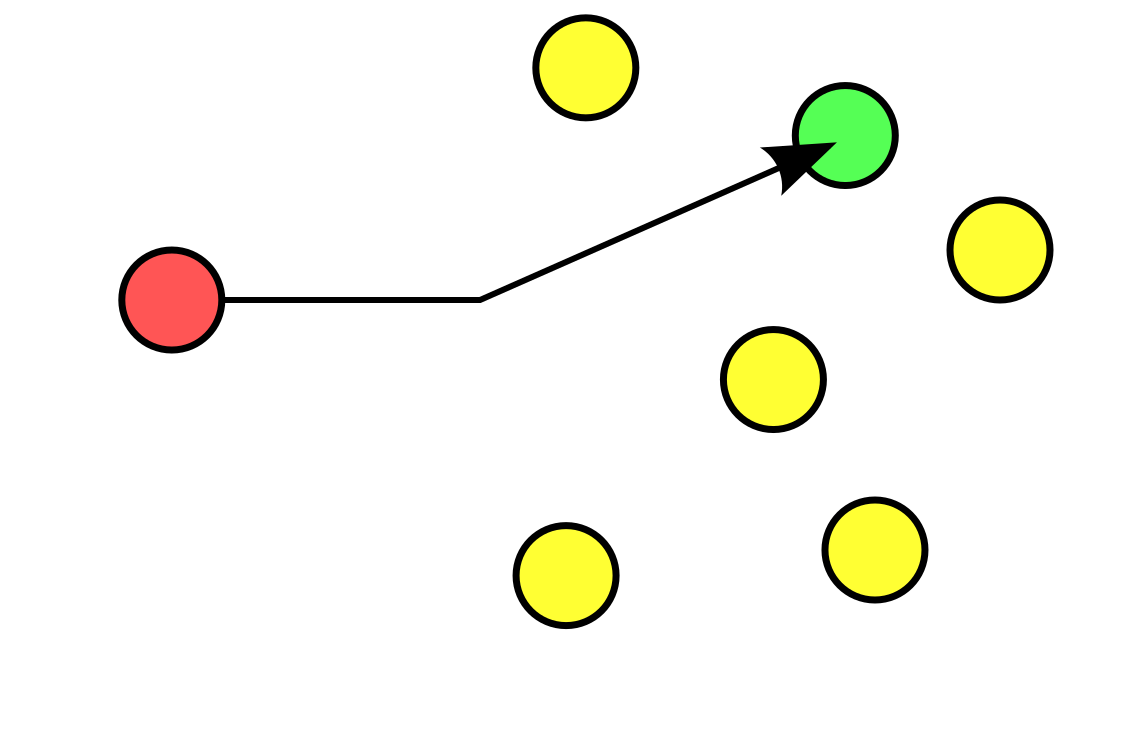
\includegraphics[width=\linewidth]{Unicast}
\end{figure}
\end{frame}

\begin{frame}{Roteamentos}
Multicast
\begin{figure}
	\includegraphics[width=\linewidth]{Multicast}
\end{figure}
\end{frame}

\begin{frame}{Roteamentos}
Broadcast
\begin{figure}
	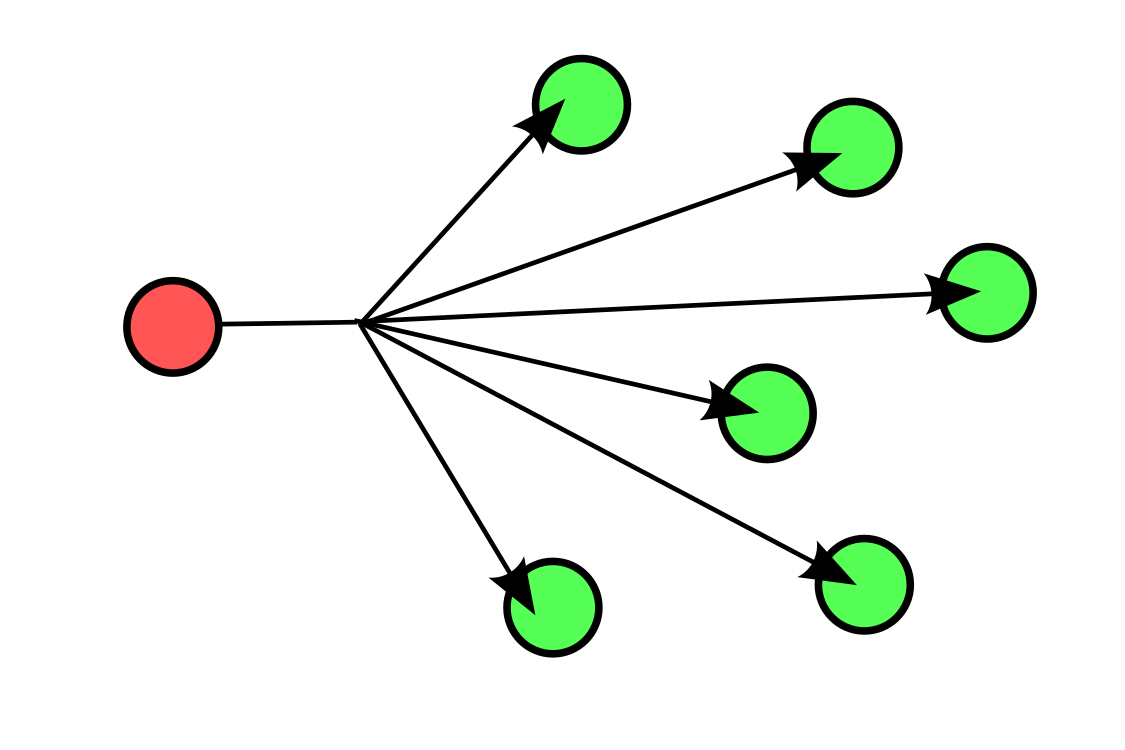
\includegraphics[width=\linewidth]{Broadcast}
\end{figure}
\end{frame}

\begin{frame}{Roteamentos}
Anycast
\begin{figure}
	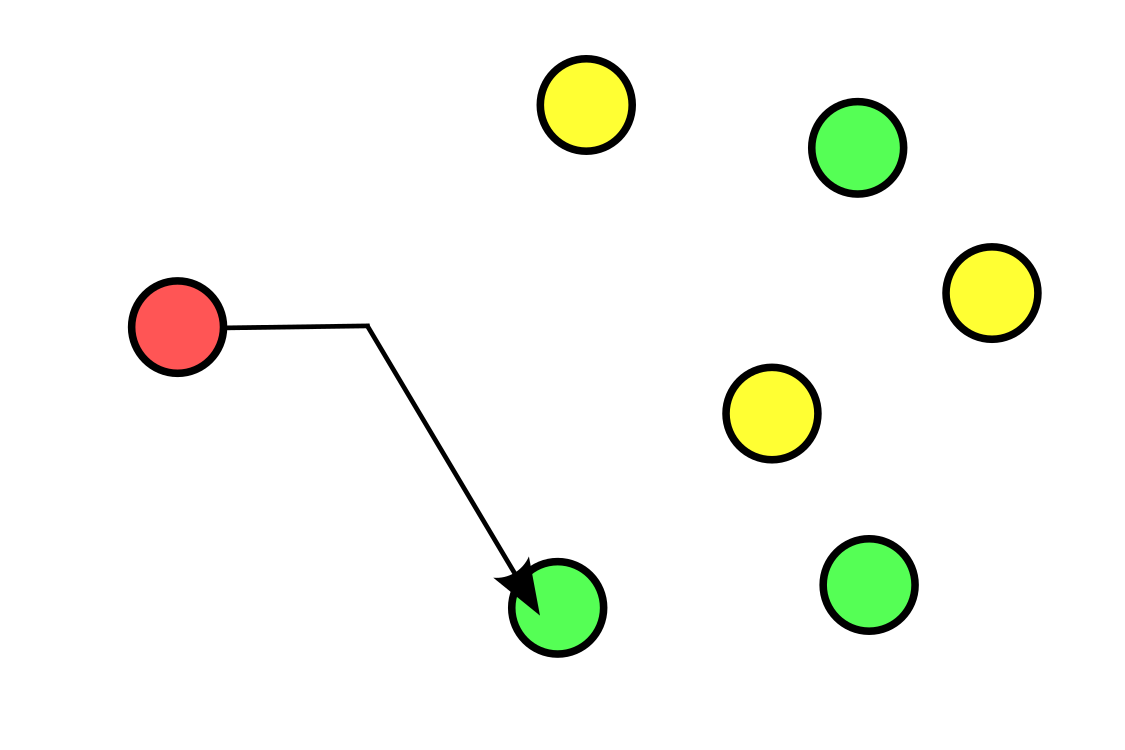
\includegraphics[width=\linewidth]{Anycast-BM}
\end{figure}
\end{frame}


\begin{frame}{Roteamentos}
Geocast
\begin{figure}
	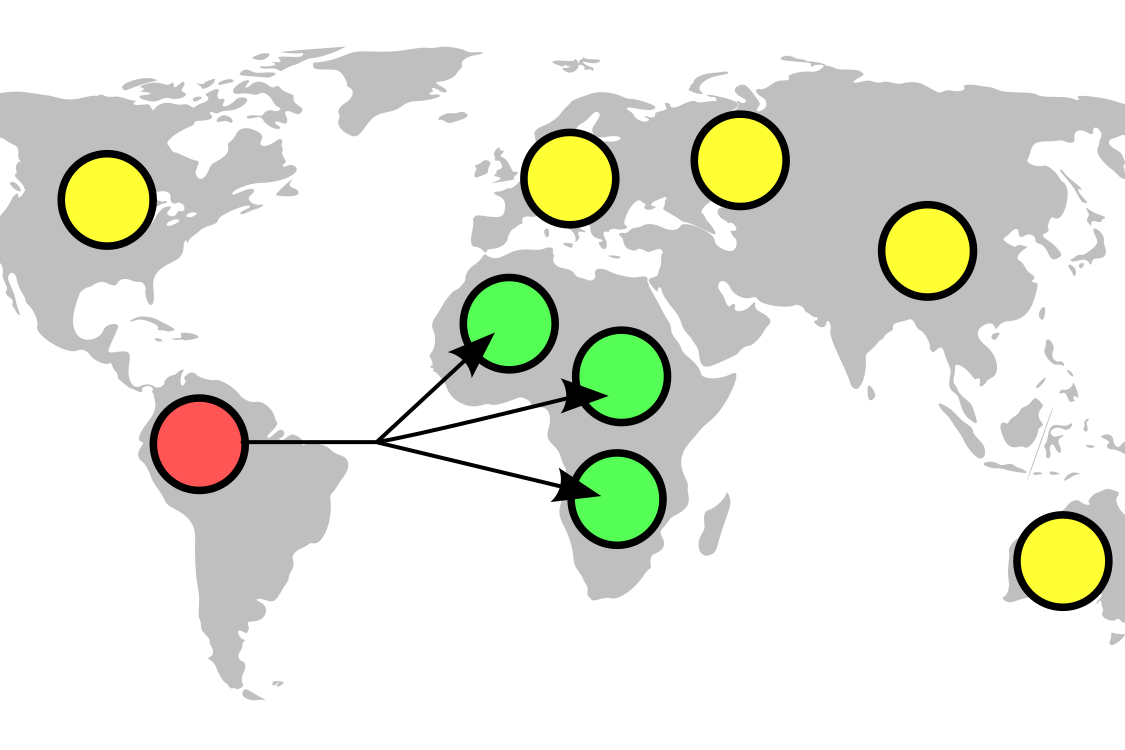
\includegraphics[width=\linewidth]{Geocast}
\end{figure}
\end{frame}

\section{Protocolos}

\begin{frame}{Protocolos}
O que são protocolos?!
\begin{itemize}
	\item Conjunto de regras
	\begin{itemize}
		\item Sintaxe
		\item Semântica
		\item Sincronização
		\item Correção de erros
	\end{itemize}
\end{itemize}
\bigskip
\begin{quotation}
	``Protocolos são para a comunicação o que as linguagens de programação são para a computação.'' (Comer, 2000)
\end{quotation}
\end{frame}

\begin{frame}{Protocolos}
Exemplos
\begin{itemize}
	\item MAC
	\item IP
	\item TCP
	\item UDP
	\item HTTP
	\item MQTT
	\item CoAP
\end{itemize}
\end{frame}

\begin{frame}{Protocolos}
MQTT
\begin{figure}
	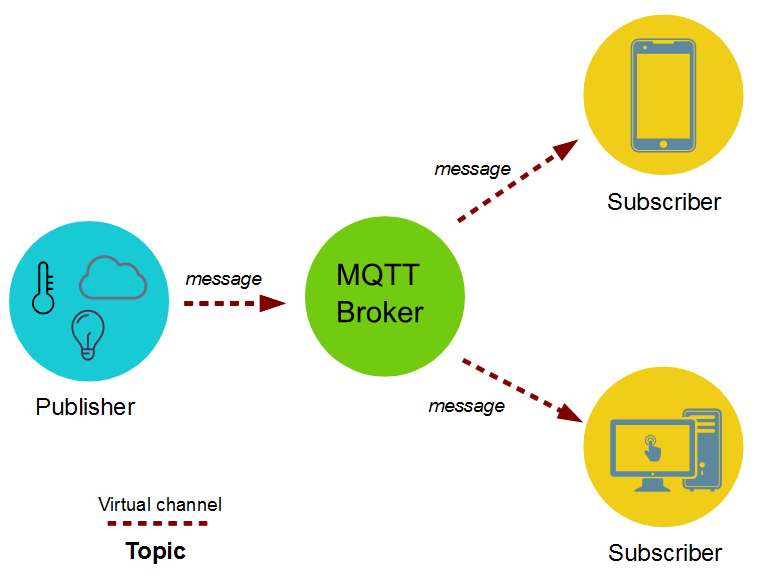
\includegraphics[width=0.8\linewidth]{mqtt_publisher_subscriber}
\end{figure}
\end{frame}

\begin{frame}{Protocolos}
CoAP
\begin{figure}
	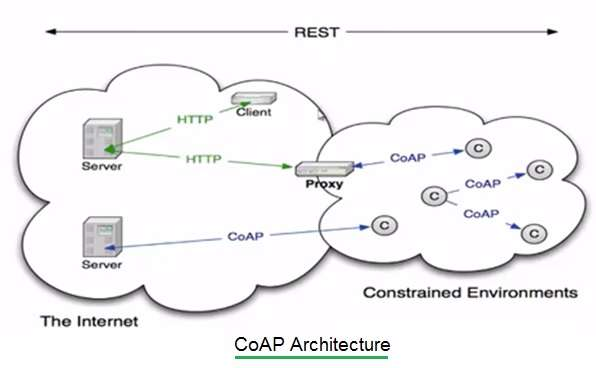
\includegraphics[width=\linewidth]{CoAP-Architecture}
\end{figure}
\end{frame}

\section{Serviços}

\begin{frame}{Serviços para troca de informações}
Tipos de serviços para troca de informações:
\begin{itemize}
	\item Serviços locais
	\item Web services
	\item Cloud services
\end{itemize}
\end{frame}

\begin{frame}{Serviços para troca de informações}
Serviços locais
\begin{itemize}
	\item Unicast, Broadcast, Multicast
	\item mDNS (Bonjour, zeroconf)
	\item UPnP (Universal Plug and Play) 
	\item DLNA (Digital Living Network Alliance)
\end{itemize}
\end{frame}

\begin{frame}{Serviços para troca de informações}
Web Services
\begin{itemize}
	\item Usados na integração com aplicações Web
	\item Tecnologias relacionadas:
	\begin{itemize}
		\item Uso de padrões Json, XML, SOAP, WSDL e UDDI
		\item AJAX
		\item Arquitetura REST (Representational State Transfer)
		\item Framework Swagger	
	\end{itemize}	
\end{itemize}
\end{frame}

\begin{frame}{Serviços para troca de informações}
Cloud Services
\begin{itemize}
	\item Usados na integração com a nuvem
	\item Tecnologias relacionadas:
	\begin{itemize}
		\item SaaS (Software as a Service)
		\item PaaS (Platform as a Service)
		\item IaaS (Infrastructure as a Service)
		\item MaaS (Monitoring as a Service)
		\item CaaS (Communication as a Service)
		\item DaaS (Data as a Service)
		\item XaaS (Anything as a Service)
	\end{itemize}	
\end{itemize}
\end{frame}

\frame{\titlepage}

\end{document}
